\documentclass[12pt, a4paper]{article}
\usepackage{amsmath}
\usepackage{amssymb}
\usepackage[margin=1in]{geometry}
\usepackage{graphicx}
\usepackage{tikz}

\title{New Problems in Entropy}
\author{Gemini}
\date{\today}

\begin{document}
\maketitle

\section{Problem 1: Heating a Gas at Constant Volume}

\subsection*{Question}
A rigid, sealed container with a volume of 50 litres holds 2.0 moles of helium, a monatomic ideal gas, at an initial pressure of $1.5 \times 10^5$ Pa. The container is heated until the pressure triples. Calculate the change in entropy of the helium gas.

\begin{center}
    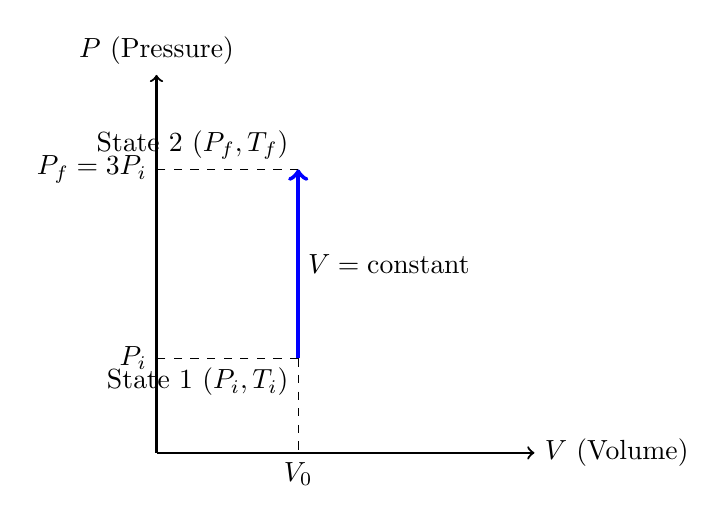
\begin{tikzpicture}[scale=1.2]
        % Axes
        \draw[->, thick] (0,0) -- (4,0) node[right] {$V$ (Volume)};
        \draw[->, thick] (0,0) -- (0,4) node[above] {$P$ (Pressure)};
        
        % Isochoric process
        \draw[->, ultra thick, blue] (1.5, 1) -- (1.5, 3);
        
        % Labels
        \node[below left] at (1.5, 1) {State 1 ($P_i, T_i$)};
        \node[above left] at (1.5, 3) {State 2 ($P_f, T_f$)};
        \node[right] at (1.5, 2) {$V = \text{constant}$};
        
        % Dashed lines to axes
        \draw[dashed] (1.5, 1) -- (0, 1) node[left] {$P_i$};
        \draw[dashed] (1.5, 3) -- (0, 3) node[left] {$P_f=3P_i$};
        \draw[dashed] (1.5, 1) -- (1.5, 0) node[below] {$V_0$};
    \end{tikzpicture}
\end{center}

\subsection*{Explanation and Solution}
This problem involves an \textbf{isochoric (constant volume)} process. Since the volume is constant, the change in entropy is calculated using the molar heat capacity at constant volume, $C_v$. For a monatomic ideal gas like helium, $C_v = \frac{3}{2}R$. We can use the Ideal Gas Law ($PV=nRT$) to find the relationship between the initial and final temperatures.

\begin{enumerate}
    \item \textbf{Identify the process and knowns:}
    \begin{itemize}
        \item Process: Isochoric ($V_i = V_f$)
        \item $n = 2.0$ mol
        \item $P_f = 3 \times P_i$
        \item Gas: Monatomic, so $C_v = \frac{3}{2}R$
    \end{itemize}

    \item \textbf{Find the temperature ratio:}
    Using the Ideal Gas Law, since $n$, $V$, and $R$ are constant, pressure is directly proportional to temperature ($P \propto T$).
    $$ \frac{P_i}{T_i} = \frac{P_f}{T_f} \implies \frac{T_f}{T_i} = \frac{P_f}{P_i} = 3 $$

    \item \textbf{Calculate the change in entropy ($\Delta S$):}
    Use the formula for entropy change in an isochoric process:
    $$ \Delta S = nC_v \ln\left(\frac{T_f}{T_i}\right) $$
    $$ \Delta S = (2.0 \text{ mol}) \times \left(\frac{3}{2} R\right) \times \ln(3) $$
    $$ \Delta S = 3 \times (8.314 \text{ J mol}^{-1}\text{K}^{-1}) \times \ln(3) $$
    $$ \Delta S \approx 24.942 \times 1.0986 $$
    $$ \Delta S \approx 27.4 \text{ J K}^{-1} $$
\end{enumerate}

\textbf{The change in entropy of the helium gas is approximately 27.4 J/K.}

\newpage

\section{Problem 2: Irreversible Energy Dissipation}
\subsection*{Question}
A 500 g block of wood is dropped from a height of 20 m. It hits the ground and comes to a complete stop. Assuming all of its initial mechanical energy is converted into thermal energy that heats the ground, calculate the entropy change of the ground if its temperature remains constant at $15^{\circ}C$.

\begin{center}
    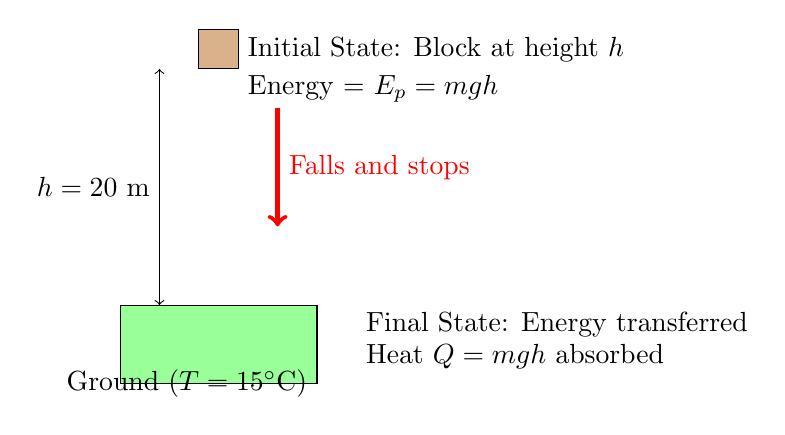
\begin{tikzpicture}
        % Initial state
        \draw[fill=brown!60] (0, 3) rectangle (0.5, 3.5);
        \node[right] at (0.5, 3.25) {Initial State: Block at height $h$};
        \node[right] at (0.5, 2.75) {Energy = $E_p = mgh$};
        \draw[<->] (-0.5, 0) -- (-0.5, 3) node[midway, left] {$h=20$ m};
        
        % Arrow for falling
        \draw[->, ultra thick, red] (1, 2.5) -- (1, 1) node[midway, right] {Falls and stops};
        
        % Final state
        \draw[fill=green!40] (-1, 0) rectangle (1.5, -1) node[left] {Ground ($T=15^\circ$C)};
       % \draw[fill=brown!60] (1.5, 0) rectangle (2, -0.2);
        \node[right] at (2, -0.25) {Final State: Energy transferred};
        \node[right] at (2, -0.65) {Heat $Q=mgh$ absorbed};
    \end{tikzpicture}
\end{center}

\subsection*{Explanation and Solution}
This is an irreversible process where macroscopic, ordered energy (gravitational potential energy) is converted into disordered thermal energy (heat). The First Law of Thermodynamics tells us that the total energy lost by the block is gained by the ground as heat, $Q$. We can then use the fundamental definition of entropy change for a reservoir at a constant temperature.

\begin{enumerate}
    \item \textbf{Calculate the initial potential energy:}
    The initial gravitational potential energy ($E_p$) of the block is the total energy that will be dissipated as heat ($Q$) upon impact.
    \begin{itemize}
        \item $m = 500 \text{ g} = 0.5$ kg
        \item $h = 20$ m
        \item $g \approx 9.81 \text{ m/s}^2$
    \end{itemize}
    $$ Q = E_p = mgh $$
    $$ Q = (0.5 \text{ kg}) \times (9.81 \text{ m s}^{-2}) \times (20 \text{ m}) = 98.1 \text{ J} $$

    \item \textbf{Calculate the entropy change of the surroundings (the ground):}
    The ground acts as a thermal reservoir at a constant temperature.
    \begin{itemize}
        \item $T = 15^{\circ}C = 15 + 273.15 = 288.15 \text{ K}$
    \end{itemize}
    The heat $Q$ is absorbed by the ground.
    $$ \Delta S_{ground} = \frac{Q}{T} $$
    $$ \Delta S_{ground} = \frac{98.1 \text{ J}}{288.15 \text{ K}} $$
    $$ \Delta S_{ground} \approx 0.340 \text{ J K}^{-1} $$
\end{enumerate}

\textbf{The entropy change of the ground is approximately 0.340 J/K.}

\newpage

\section{Problem 3: Rate of Entropy Change in Conduction}
\subsection*{Question}
A large single-pane glass window is 2.0 m tall, 1.5 m wide, and 4.0 mm thick. On a cold day, the temperature of the inner surface of the glass is $12^{\circ}C$ and the temperature of the outer surface is $-5.0^{\circ}C$. Calculate the total rate of entropy change for the system (the window and its thermal reservoirs). The thermal conductivity of glass is $0.80 \text{ W m}^{-1}\text{K}^{-1}$.

\begin{center}
    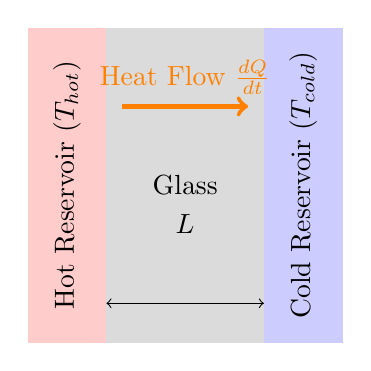
\begin{tikzpicture}
        % Reservoirs
        \fill[red!20] (-1,-2) rectangle (0,2);
        \node[rotate=90] at (-0.5, 0) {Hot Reservoir ($T_{hot}$)};
        
        \fill[blue!20] (2,-2) rectangle (3,2);
        \node[rotate=90] at (2.5, 0) {Cold Reservoir ($T_{cold}$)};
        
        % Window Pane
        \fill[gray!40, opacity=0.7] (0,-2) rectangle (2,2);
        \node at (1,0) {Glass};
        \node at (1,-0.5) {$L$};
        \draw[<->] (0,-1.5) -- (2,-1.5);
        
        % Heat Flow Arrow
        \draw[->, ultra thick, orange] (0.2, 1) -- (1.8, 1) node[midway, above] {Heat Flow $\frac{dQ}{dt}$};
    \end{tikzpicture}
\end{center}

\subsection*{Explanation and Solution}
This is a steady-state heat conduction problem. Heat flows continuously from the warm interior to the cold exterior through the glass. The total rate of entropy change is the sum of the rates for the hot reservoir (inside air, losing heat) and the cold reservoir (outside air, gaining heat). Since the process is in a steady state, the entropy of the window itself is not changing.

\begin{enumerate}
    \item \textbf{Identify values and convert to SI units:}
    \begin{itemize}
        \item Area $A = 2.0 \text{ m} \times 1.5 \text{ m} = 3.0 \text{ m}^2$
        \item Thickness $L = 4.0 \text{ mm} = 0.004 \text{ m}$
        \item $k = 0.80 \text{ W m}^{-1}\text{K}^{-1}$
        \item $T_{hot} = 12^{\circ}C = 285.15 \text{ K}$
        \item $T_{cold} = -5.0^{\circ}C = 268.15 \text{ K}$
    \end{itemize}

    \item \textbf{Calculate the rate of heat flow ($\frac{dQ}{dt}$):}
    Using Fourier's Law of heat conduction:
    $$ \frac{dQ}{dt} = \frac{kA(T_{hot} - T_{cold})}{L} $$
    $$ \frac{dQ}{dt} = \frac{(0.80) \times (3.0) \times (285.15 - 268.15)}{0.004} $$
    $$ \frac{dQ}{dt} = \frac{(0.80) \times (3.0) \times (17.0)}{0.004} = 10200 \text{ W (J/s)} $$

    \item \textbf{Calculate the total rate of entropy change:}
    The total rate is the sum of the rates for the hot reservoir (negative change) and the cold reservoir (positive change).
    $$ \frac{dS_{total}}{dt} = \frac{dS_{hot}}{dt} + \frac{dS_{cold}}{dt} $$
    $$ \frac{dS_{total}}{dt} = \left(-\frac{1}{T_{hot}}\frac{dQ}{dt}\right) + \left(\frac{1}{T_{cold}}\frac{dQ}{dt}\right) $$
    $$ \frac{dS_{total}}{dt} = \frac{dQ}{dt} \left(\frac{1}{T_{cold}} - \frac{1}{T_{hot}}\right) $$
    $$ \frac{dS_{total}}{dt} = 10200 \left(\frac{1}{268.15} - \frac{1}{285.15}\right) $$
    $$ \frac{dS_{total}}{dt} = 10200 \left(0.0037292 - 0.0035069\right) $$
    $$ \frac{dS_{total}}{dt} = 10200 \times (0.0002223) \approx 2.27 \text{ W K}^{-1} $$
\end{enumerate}

\textbf{The total rate of entropy change for the system is approximately 2.27 W/K.}

\end{document}